%!TEX root = ../paper.tex
\section{Discussions}
\label{sec:energy}

In this section we discuss (a) the energy implications of changing the clock speed, and (2) a possible Web page optimization for low-end devices based on our observations in \S\ref{label:web}.

\begin{figure}[t]
  \centering
  \subfloat[Youtube and Skype]{
  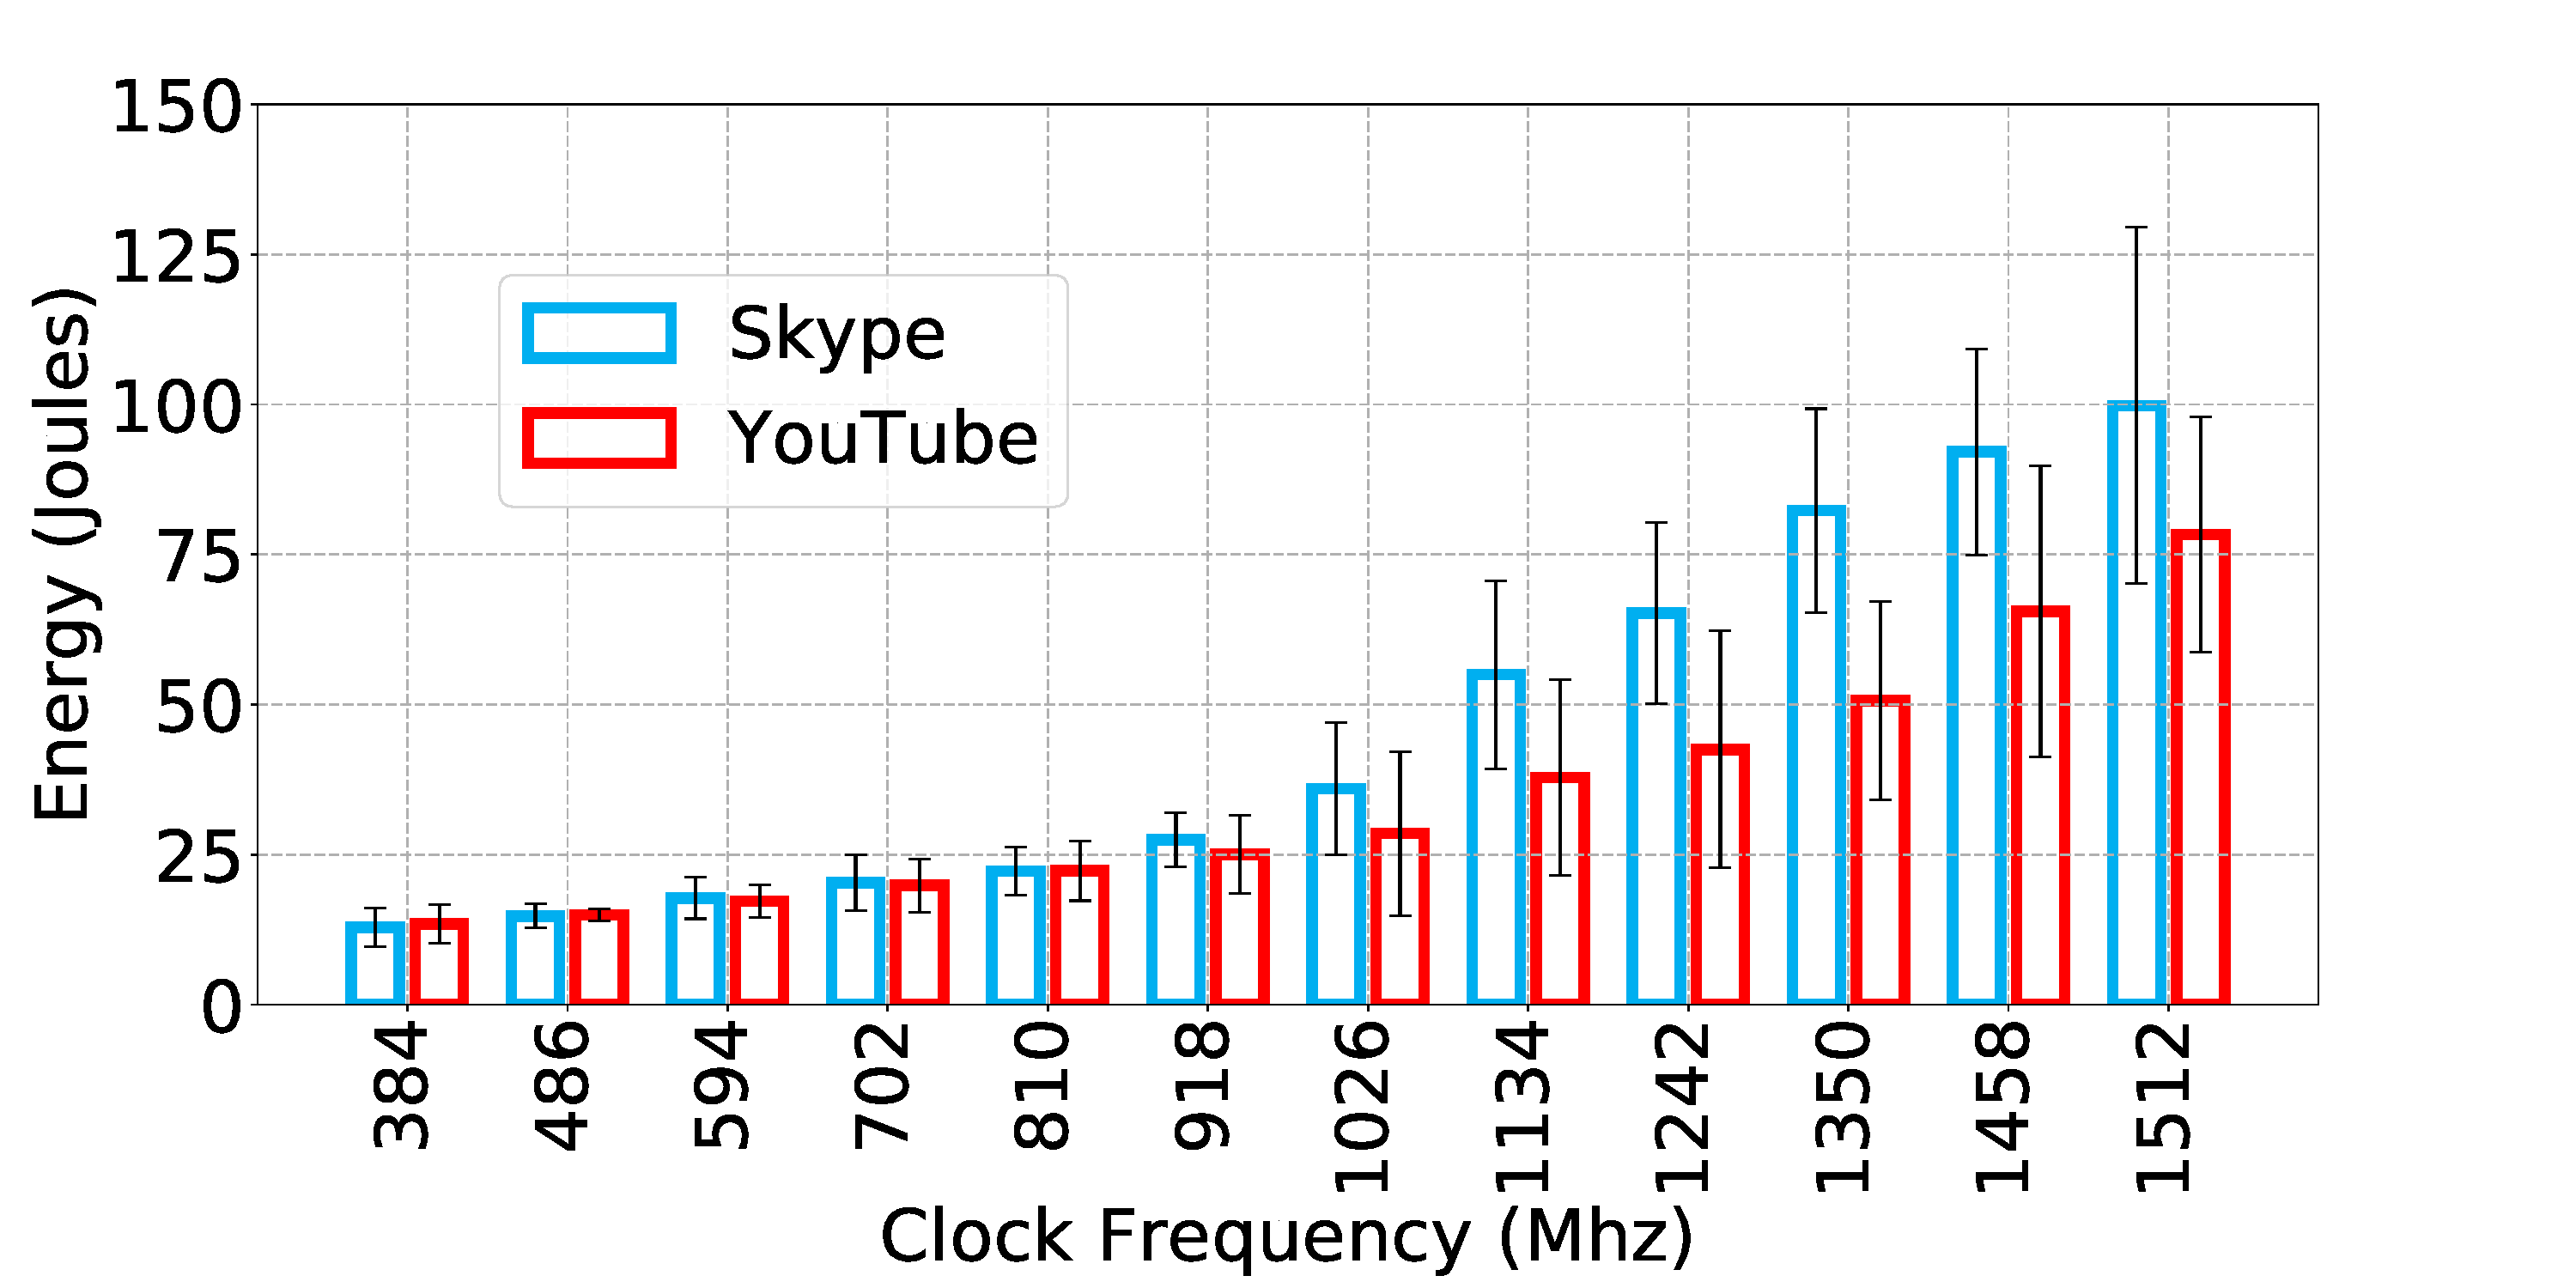
\includegraphics[width=0.9\linewidth]{sections/power-video}}
  
%    \caption{\textit{Energy vs. Clock during Webpage loads.}}
%   \vspace{-0.15in}
% \label{fig:power-web}
\subfloat[Web page load]{
  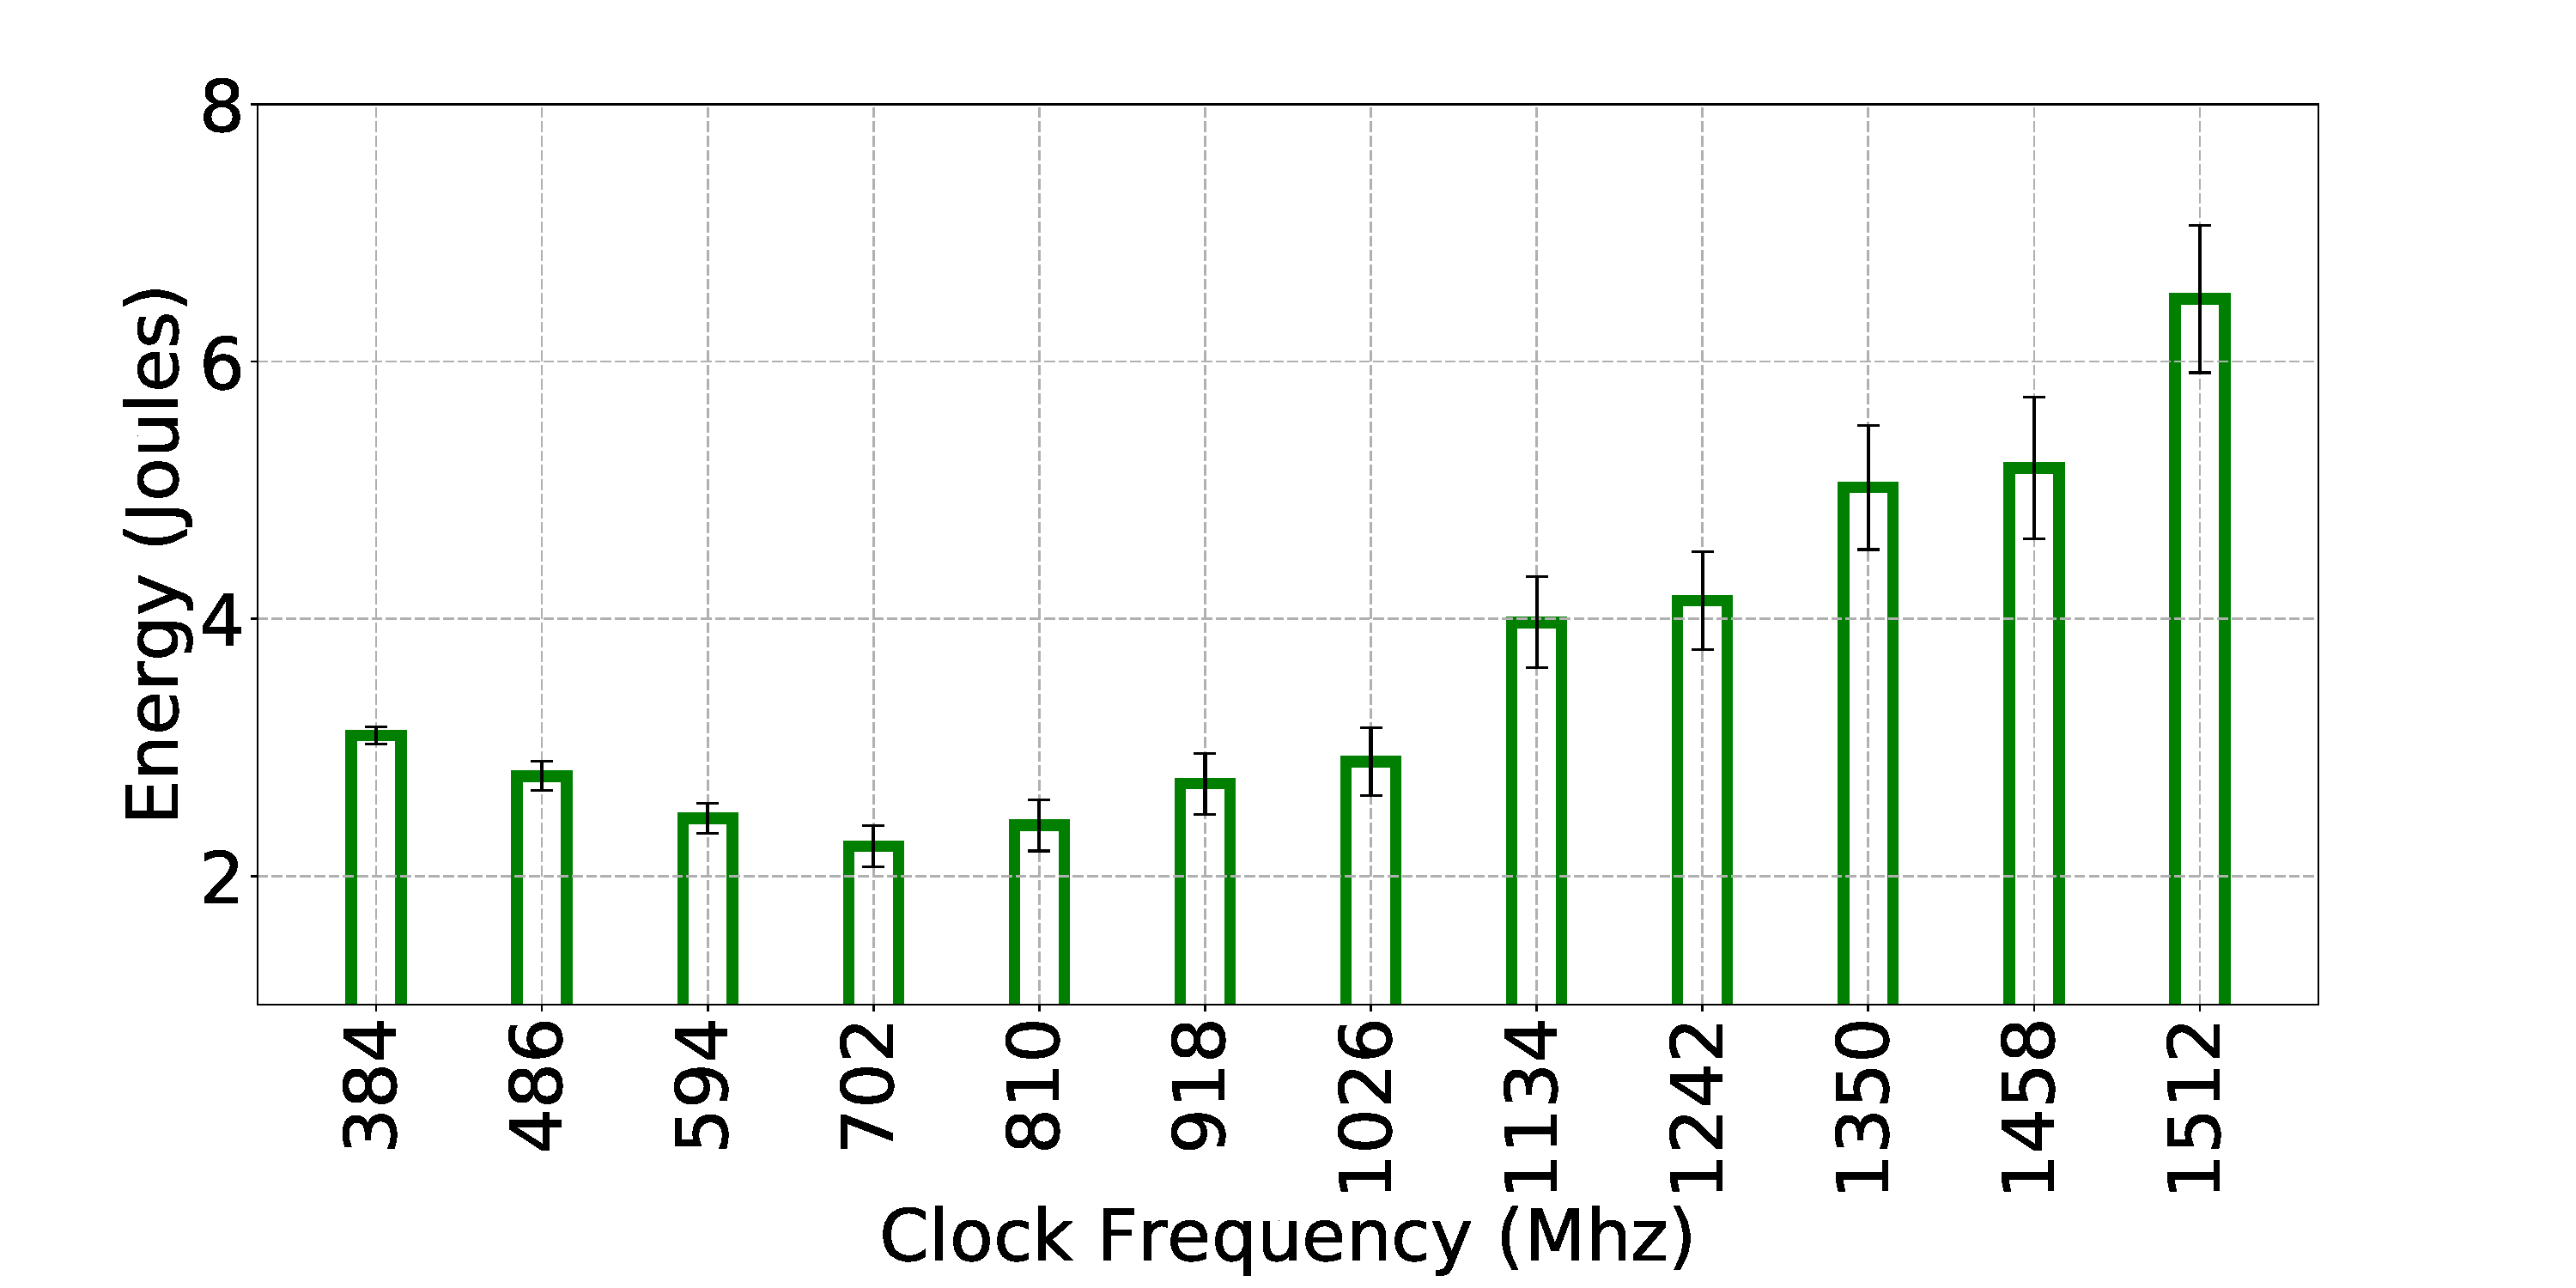
\includegraphics[width=0.9\linewidth]{sections/power-plt}
  }
  \caption{Energy consumption vs. clock rate for
  (a) video streaming and telephony and (b) Web page load}
   %\vspace{-0.15in}
\label{fig:power-video-web}
\end{figure}

% \begin{figure}[t]
%   \centering
%   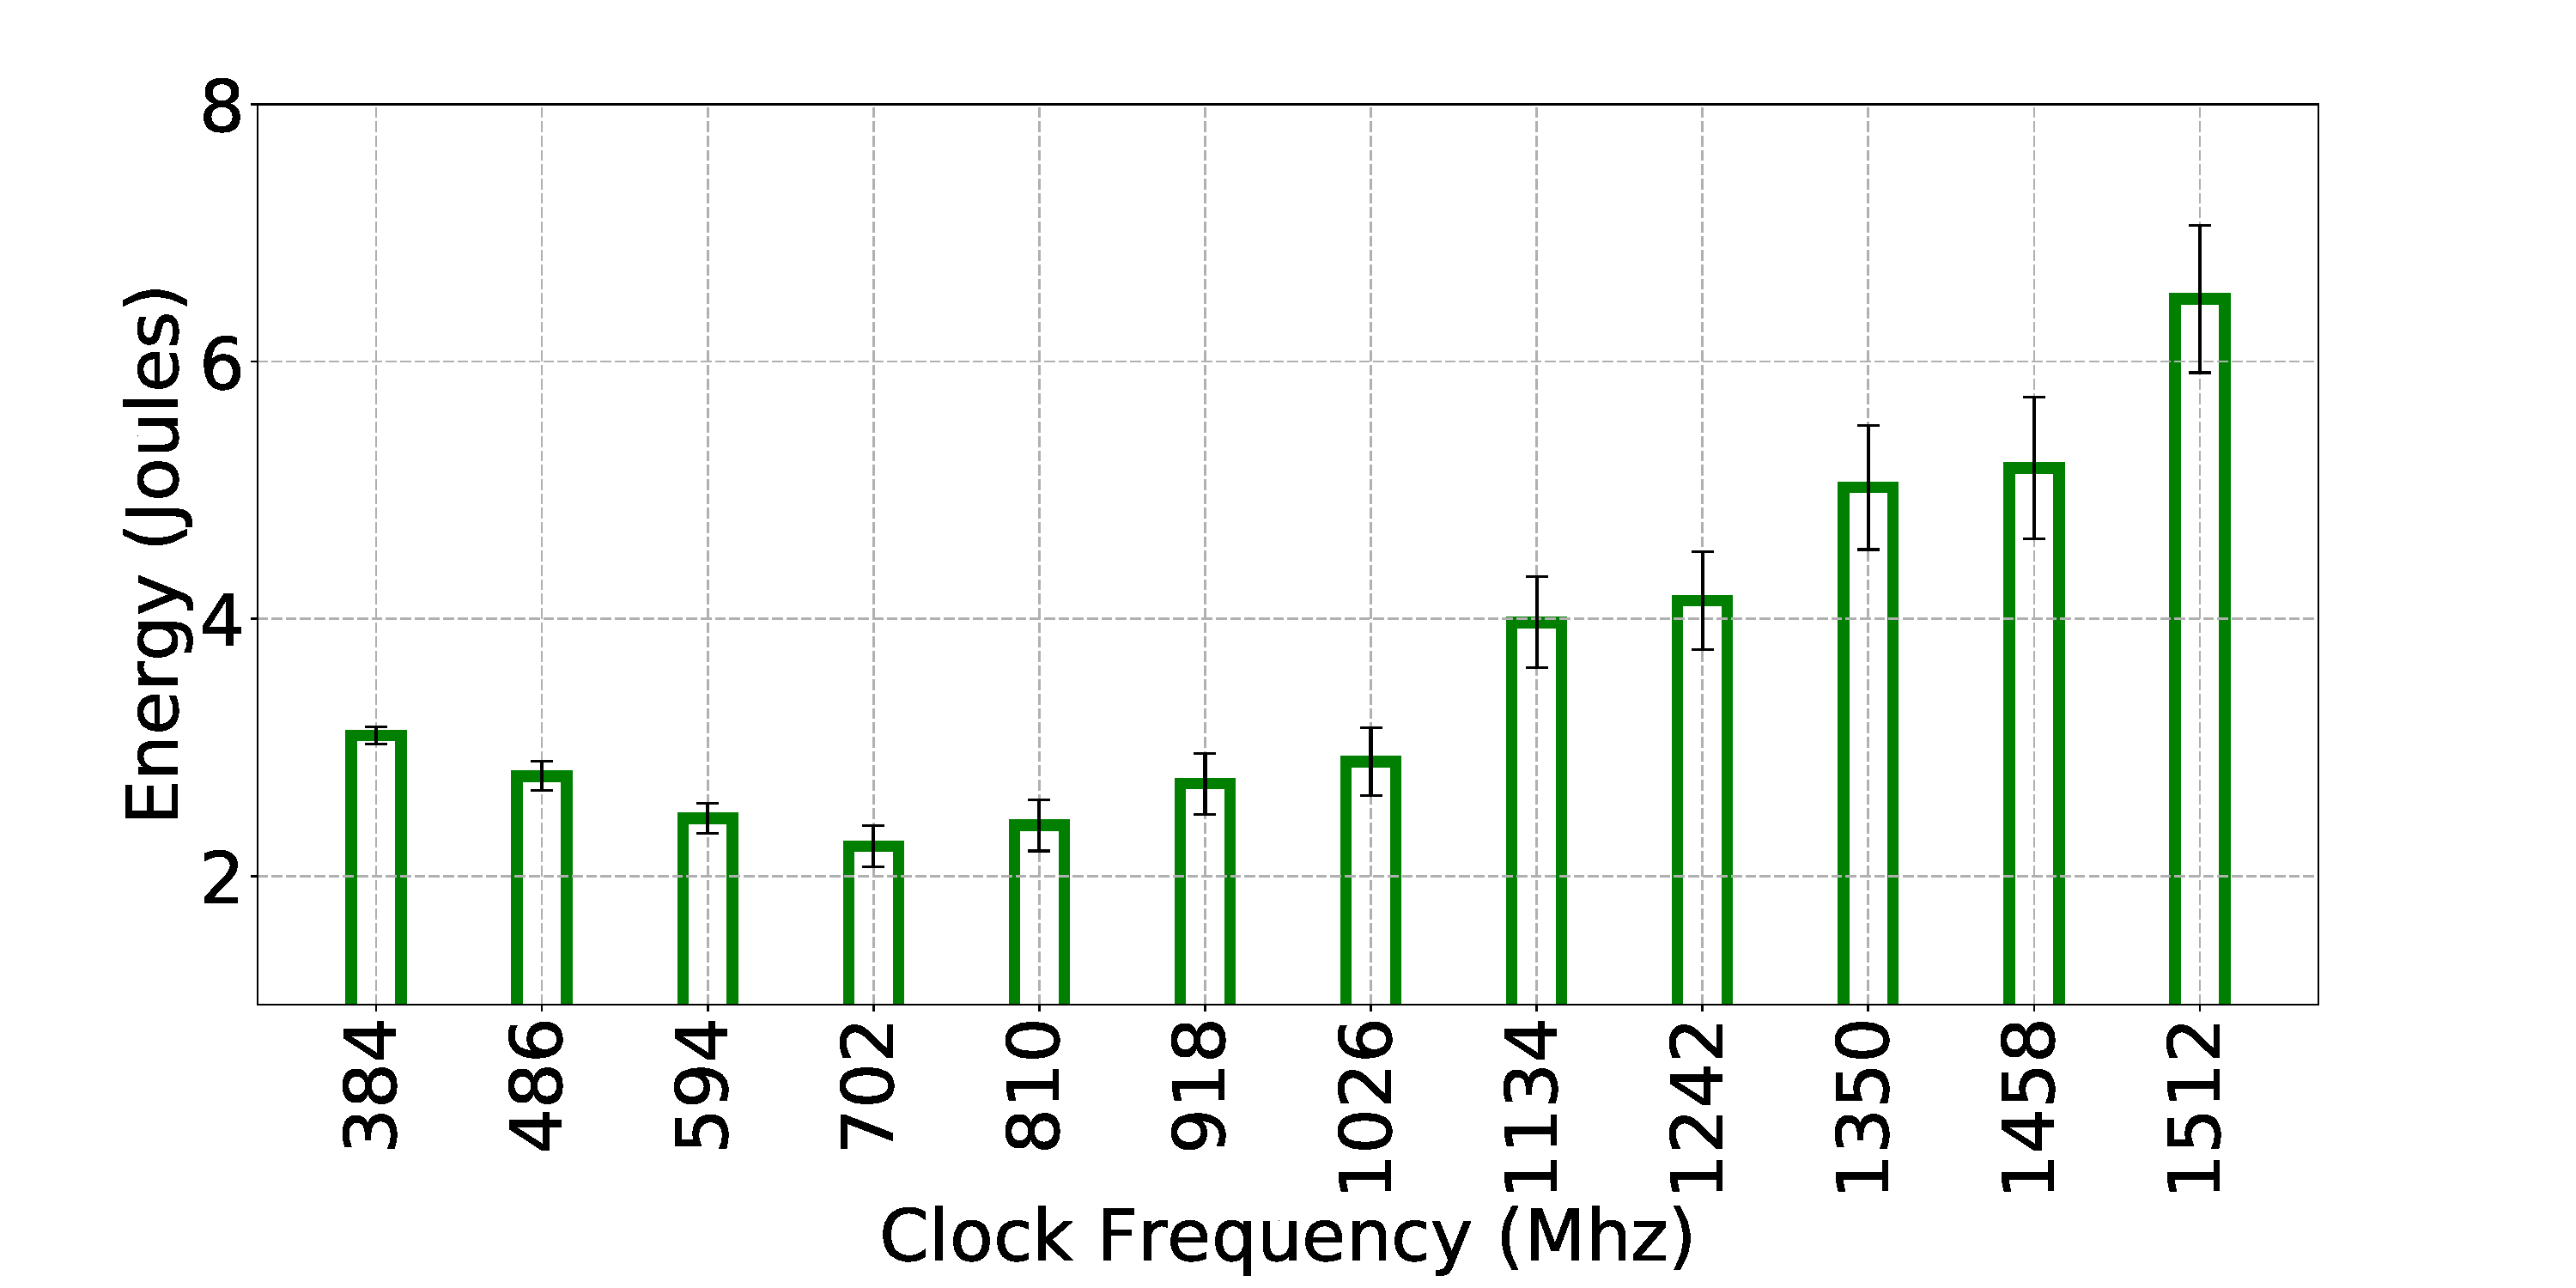
\includegraphics[width=\linewidth]{sections/power-plt}
%     \caption{\textit{Energy vs. Clock during Webpage loads.}}
%    \vspace{-0.15in}
%   \label{fig:power-web}
% \end{figure}
% \begin{figure}[t]
%   \centering
%   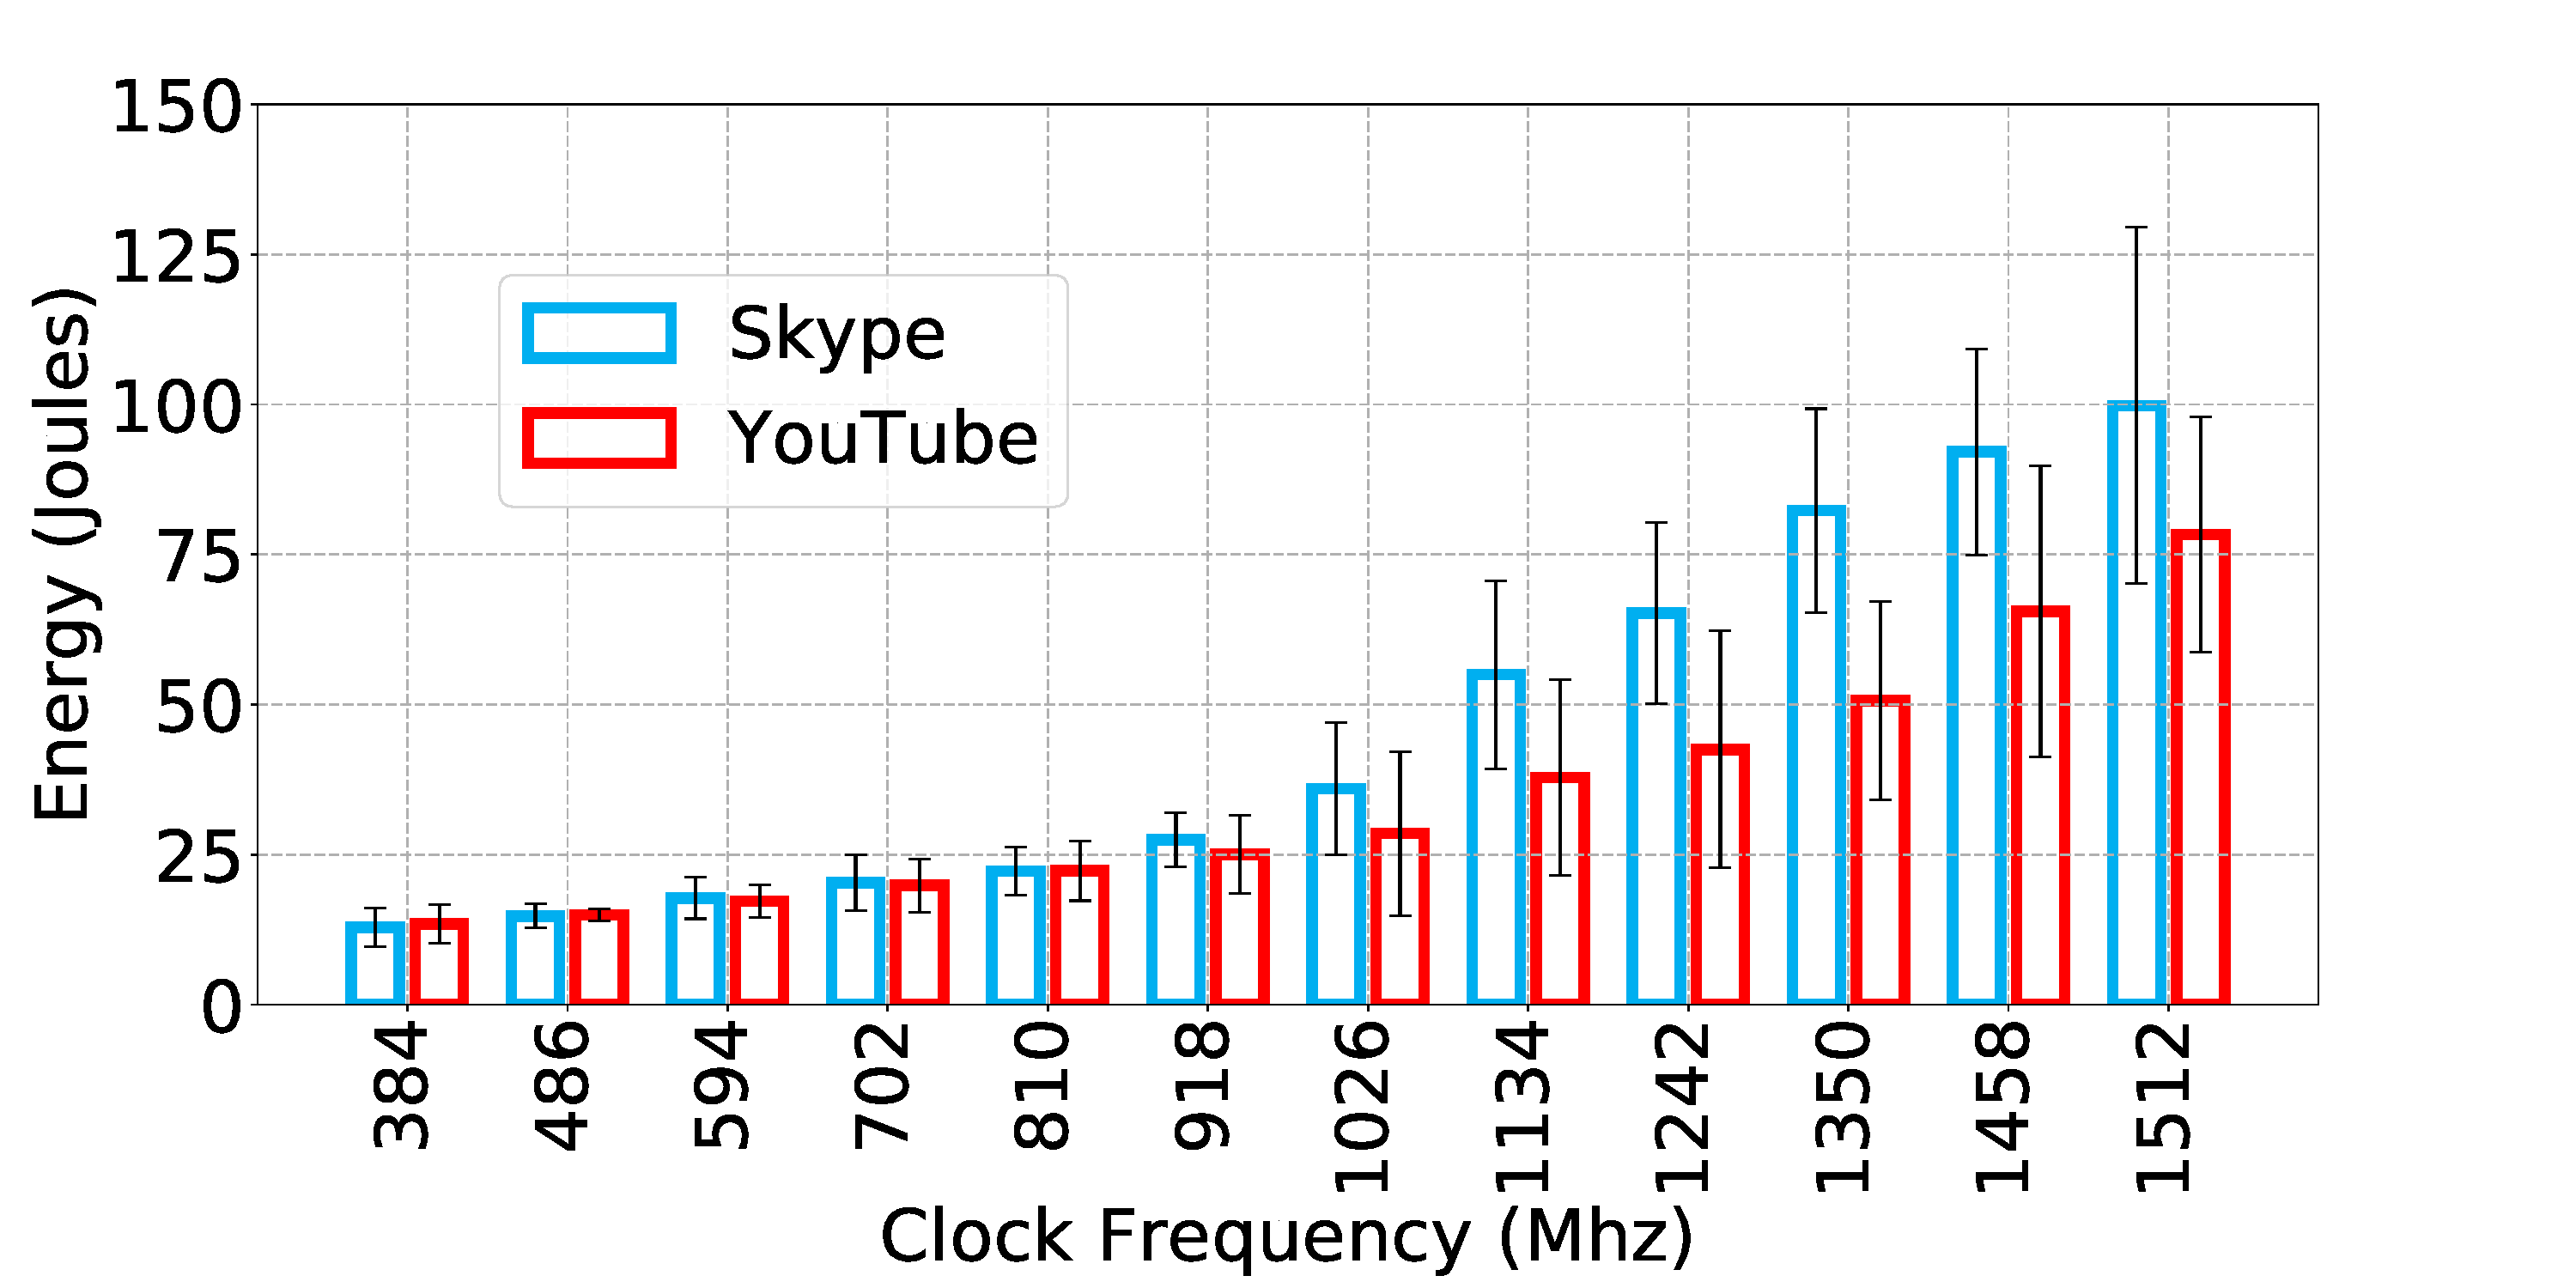
\includegraphics[width=\linewidth]{sections/power-video}
%   \caption{\textit{Energy vs. Clock during Skype and YouTube. More than 80\% of increase in YouTube and Skype energy consumption respectively.}}
%    \vspace{-0.15in}
%   \label{fig:power-video}
% \end{figure}

\subsection{Energy Consumption}
CPU clock frequency has an impact on the device's energy consumption and here low end devices may win. To evaluate 
energy consumption we use the same set up as the one described in \S\ref{sec:setup}. The experiments are conducted on the Nexus 4 phone and we use the Snapdragon Profiler~\cite{qualsnap} to log the energy consumption. The profiler samples energy at a high sampling rate of 20 times a second. %energy consumption \todo{do we know anything about the accuracy of the profiler?}. \mallesh{The profiler has different sampling rates (50ms, 120ms, 240ms) at which the metrics can be collected. We use minimum value 50ms.}

Figure~\ref{fig:power-video-web}
shows the energy consumption for all three applications
considered in this study with increasing 
clock frequency. Figure~\ref{fig:power-video-web}(a) shows the energy consumption while running YouTube and Skype at different frequencies. With increase in CPU clock frequency energy consumption increases steadily - somewhat faster for telephony (Skype) than streaming (YouTube). One reason for this is that YouTube prefetches video content. This allows the network to be inactive after the required content is prefetched. But Skype is interactive requiring that the network remain active throughout the session. 
%\mallesh{We explain this by observing that while Youtube plays videos on demand, Skype plays live video. 
%Video on demand allows prefetching of video, which helps in conserving energy since the network interface is not always active. 
%However, this is not possible for Skype, as it plays live videos and needs to always keep fetching video packets to provide continuous service.}

Overall, the energy consumptions are more
drastic than the QoE improvements in these two applications
with faster clocks. For example, from the slowest end to fastest
end of clock frequency 1) Skype consumes $7\times$ more 
energy  while providing about $2\times$ better
frame rate; 2)  YouTube provides a modest
improvement of startup latency, $\approx$1 sec vs. 
$\approx$3 sec for about a 5 min video, but consumes
$5\times$ more energy. 

For Web page load (Figure~\ref{fig:power-video-web}(b)), 
the observation is different. As CPU frequency increases, the 
energy consumption first decreases and then increases. This 
is because initially the faster page load compensates
more than the increased power draw due to faster 
clock. Recall that 
energy consumption = avg. power draw $\times$ time. Similar to the video example, energy consumption is more drastic than QoE improvement (Figure~\ref{fig:plt_clock}). % When the CPU speeds increases from 702 MHz to 1512 MHz, energy consumption increases by $3\times$ but the average PLT only decreases by 50\% by 

Thus, an optimal frequency exists if one is interested
in optimizing the energy consumption for applications. Currently, when the frequency governor~\cite{ad-governors} is set to power-saving, the application is set to use the lowest CPU frequency. Instead, one can design a governor that takes into account the marginal performance improvement and the resulting energy consumption. 

% when loading Web pages under different CPU frequencies. 
% At high frequencies, faster CPU leads to higher power consumption. et 

% When the CPU frequency is lower than 801 MHz, the energy consumption decreases going from 384 MHz to 702 MHz.This is an anomaly the faster the CPU runs, the more power it draws. In this case, the lower power consumption is because the Web page loads speed up considerably from an average of 14 seconds to 8 seconds.  

%Figure \ref{fig:power-web} shows that there is a sweet spot in the CPU speeds, where increasing the CPU speed beyond a point reduces the returns in terms of PLT, but increases the power consumption considerably. However, the governors~\cite{} in todays mobile devices \todo{I want to say something about how they work, but I am not sure of it yet.}




%%We find a difference of 4Joules of energy consumption from high clock to low clock.
%We observe that at low frequencies till 702Mhz, the energy consumption actually reduces when the frequency increases. 
%This can be explained by the fact that while increasing the frequency increases power consumption, it also reduces page load time. 
%Increasing the frequency further however increases the energy consumption. 
%This is because the increase in power consumption becomes higher and dominates the reduction in page load time. Thus, we observe a trend of super-linear increase in energy consumption with an increase in clock frequency similar to our observation for file download and video playing.



%CPU clock is one of the most important metric that impacts energy efficiency \cite{zhu2015role}. In this section, we look at the energy consumption of the above applications under different clock frequencies. We run these experiments for 20 runs. For video applications, we run the video (or call) for 2 minute duration.


 
%We observe an exponentail increase of 88Joules and 64 Joules of energy from high clock to low clock in Skype and YouTube respectively.
%The energy is linearly increased till 918Mhz and then an exponential increase in energy consumption until high clock under both YouTube and Skype.
%However, the energy consumption of Skype increases much faster than that of Youtube. 
%We explain this by observing that while Youtube plays videos on demand, Skype plays live video. 
%Video on demand allows prefetching of video, which helps in conserving energy since the network interface is not always active. 
%However, this is not possible for Skype, as it plays live videos and needs to always keep fetching video packets to provide continuous service.

